\documentclass{standalone}
\usepackage[T1]{fontenc}
\usepackage[utf8]{inputenc}
\usepackage{pgf,tikz}
\usepackage{setspace}
\usepackage{pgfplots}
\pgfplotsset{compat=1.11}

\begin{document}

\def\FD{tf([1 0], [1/20, 1])}% Modified D-part

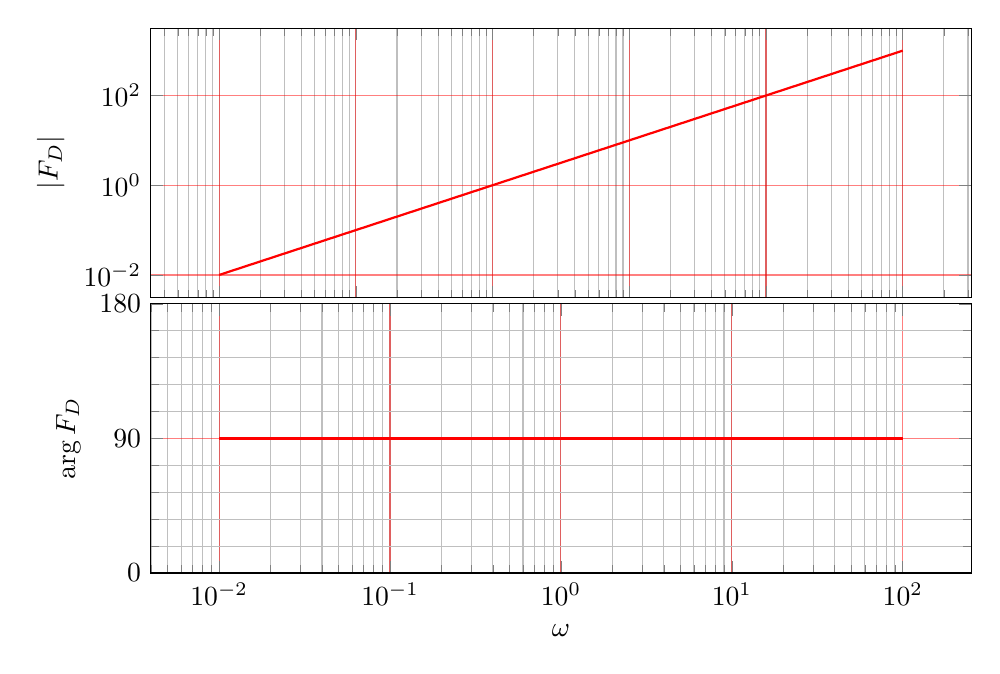
\begin{tikzpicture}
  \begin{loglogaxis} [
      width=12cm,
      height=5cm,
      ylabel=$|F_D|$,
      xticklabels=\empty,
      %ytick={},
      grid=both,
      minor y tick num=9,
%      extra y ticks={.5}, % how to convert to fixed point tick label ?
%      extra y tick style={log identify minor tick positions=true},
      every major grid/.style={red, opacity=0.5},
  ]
    %\addplot+ 
    %shell[thick, black, no marks, prefix=pgfshell_, id=bodenm] {octave -q --eval  "format long; G=\FD ; [mag,phi,w]=bode(G,{0.01,10}); disp(cat(2,w',mag))"};
    \addplot+ [thick, red, no marks, domain=0.01:1000, samples=400] {x};
  \end{loglogaxis}
  \begin{semilogxaxis} [
      xlabel=$\omega$,
      ylabel=$\arg F_D$,
      yshift = -3.5cm, 
      width=12cm,
      height=5cm,
      grid=both,
      ytick={ 0, 90, 180},
      ymin = 0,
      ymax = 180,
      minor y tick num=4,
      every major grid/.style={red, opacity=0.5},
      %legend entries={Bessel filter, Delay of one},
      %legend pos={south west},
  ]
    %\addplot+ 
    %shell[thick,black, no marks, prefix=pgfshell_, id=bodenm] {octave -q --eval  "format long; G=\FD ; [mag,phi,w]=bode(G,{0.01, 10}); disp(cat(2,w',phi))"};
    \addplot+ [thick, red, no marks, domain=0.01:100, samples=10] {90};
  \end{semilogxaxis}
\end{tikzpicture}

\end{document}
